\documentclass[14pt]{article}
\usepackage{listings}
\usepackage{color}
\usepackage{graphicx}
\usepackage{setspace}

\definecolor{dkgreen}{rgb}{0,0.6,0}
\definecolor{gray}{rgb}{0.5,0.5,0.5}
\definecolor{mauve}{rgb}{0.58,0,0.82}

\lstset{frame=tb,
  language=promela,
  aboveskip=3mm,
  belowskip=3mm,
  showstringspaces=false,
  columns=flexible,
  basicstyle={\small\ttfamily},
  numbers=none,
  numberstyle=\tiny\color{gray},
  keywordstyle=\color{blue},
  commentstyle=\color{dkgreen},
  stringstyle=\color{mauve},
  breaklines=true,
  breakatwhitespace=true
  tabsize=3
}







\begin{document}
\title{% 
  \huge Concurrent and Distributed Systems \\
  \vspace{20mm}
  \large Laboratory Assignment 2 \\}

\date{\today}
\maketitle
\begin{center}
\vspace{30 mm}

\title{\huge Student: Marcu Andrei Cristian}
\\\vspace{10 mm}
\title{\huge Computers and Information Technology}
\\\vspace{10 mm}
\title{\huge CEN 3.2 A}
\\\vspace{10 mm}
\title{\huge 3rd Year}
\end{center}
\date{}
\maketitle

\newpage
\section*{Problems statements}
\vspace{20 mm}
\textbf{Problem 1} (50p) \\
Implement Dekker algorithm using 2 processes (as available
in Critical Sections Laboratories).
Assignment: Implement the Dekker algorithm in Promela, describe the output
and different scenarios (in multiple executions)
\\\vspace{10 mm}\\
\textbf{Problem 2} (50p) \\
What values can n have at the end of the concurrent counting algorithm execution?
Assignment: Implement this algorithm in Promela. What values do you get at the end for n?
Assignment: Prove the above by describing in the technical reports a few test
scenarios and different states as shown in the first course.
Assignment: Describe the output and different scenarios (in multiple executions).
\begin{center}
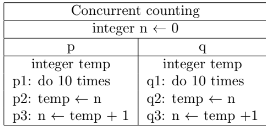
\includegraphics[height=1.8in, width = 5in]{problema2.png}\\
\end{center}
\newpage
\\\vspace{10 mm}\\
\textbf{Problem1:} Dekker algorithm is designed to solve the critical section problem. It synchronizes two threads to enter one by one in a critical section without conflict. I've used the version presented at the course. It works as follows:\\
We have two flags : wantq and wantp. When wantq is 1 the thread q wants to enter in the critical section, same for wantp.\\
We have an integer turn which can have the value 1 or 2. It saves the priority in case if both threads want to enter the critical section at the same time.
\\\vspace{20 mm}\\
\textbf{Problem2:} As we've seen in the statement we have 2 threads incrementing the same variable n 10 times. N is a global variable so it will have the same value for all threads.\\
For example the result for the input presented in the solution ( 2 threads, 10 iterations each) n will reach a random value close to 20 or exactly 20. (20 is the correct answer).\\
I'll explain more examples later on my presentation.\\
Now that we've clarified the Problems Statements we can move on to the implementation.
\newpage

\section*{Solution Problem 1}\\
\begin{lstlisting}
//----------------------------dekker.pml----------------------------
bool wantp = false, wantq = false;
byte turn = 1;

active proctype p() {
	do
	:: wantp = true;
		do
		:: wantq ->
			if
			:: (turn == 2) ->
				wantp = false; turn == 1; wantp = true
			:: else
			fi
		:: else -> break
		od;
		printf("P se afla in sectiunea critica\n");
		turn = 2;
		wantp = false
	od
}
active proctype q() {
	do
	:: wantq = true;
		do
		:: wantp ->
			if
			:: (turn == 1) ->
				wantq = false; turn == 2; wantq = true
			:: else
			fi
		:: else -> break
		od;
		printf("Q se afla in sectiunea critica\n");
		turn = 1;
		wantq = false
	od
}

\end{lstlisting}
\vspace{5 mm}\\
\newpage
\section*{Experiments and results for problem 1}
\\\\\\
\begin{center}
Even though it's an infinite loop all examples will have 250 steps.
1. Random example 1
\vspace{10mm}

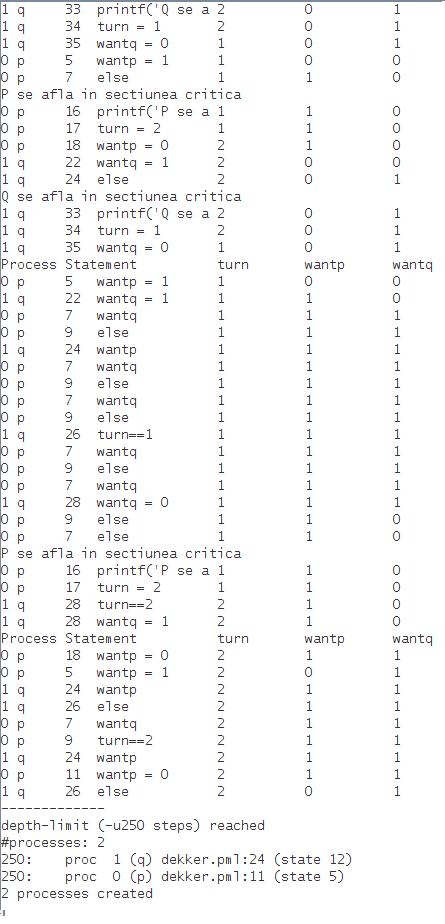
\includegraphics[height=6in, width = 4in]{dekker1.png}\\
\newpage
\end{center}\\


\newpage

\begin{center}
2. Random example 2
\vspace{10mm}

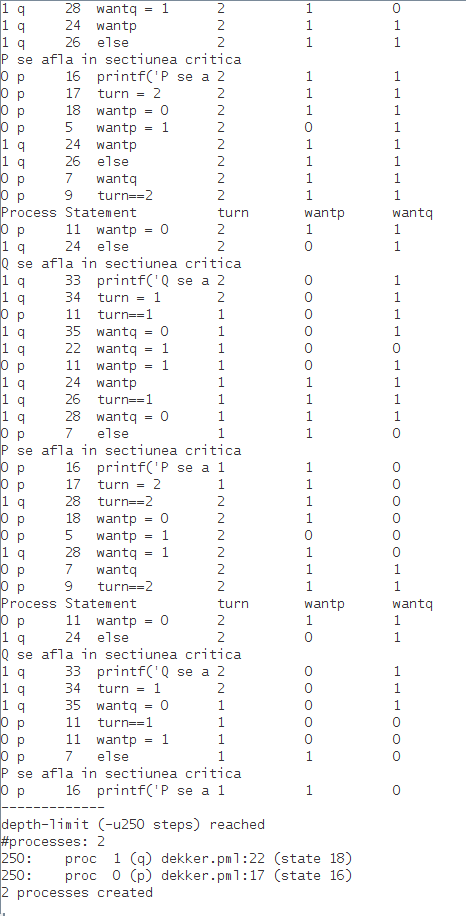
\includegraphics[height=6in, width = 4in]{dekker2.png}\\
\end{center}\\

\newpage

\begin{center}
3. Random example 3
\vspace{10mm}

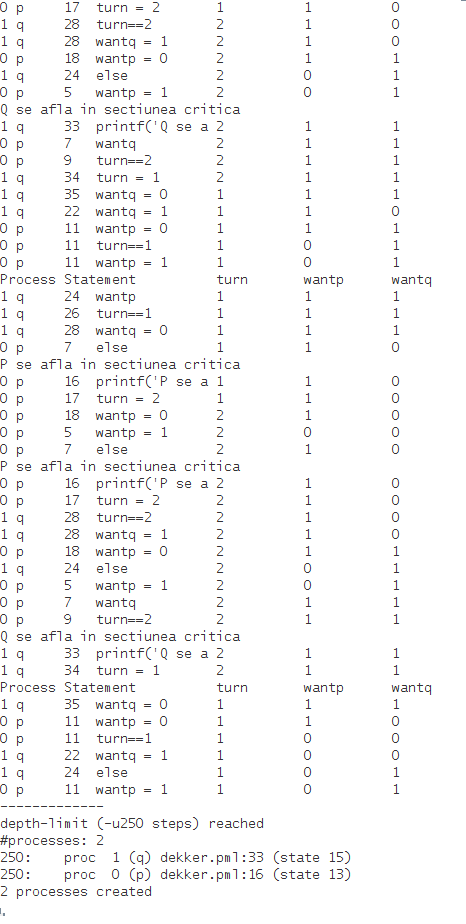
\includegraphics[height=6in, width = 4in]{dekker3.png}\\
\end{center}\\
In the examples presented before we can see only the end of the execution. Full examples will be found in the Experimental data and results folder\\
As we can see in all examples presented before, the threads enter the critical section one by one when the flag is true.


\section*{Conclusions Problem 1}
\vspace{10 mm}
Working on this problem, I have acquired lots of knowledge about thread programming, about the problems that can appear when we are using threads. Dekker algorithm is one good solution to avoid critical section problem and make two threads work with the same variable without modifiying it in the same time. The issue that Dekker algorithm avoids is presented in the second problem.
\newpage

\section*{Solution Problem 2}\\
\begin{lstlisting}
//----------------------------concurrent.pml----------------------------

int n = 0;

active[2] proctype pq() {
	int i = 0, temp;
	do
	:: i < 10 -> 
			temp = n; 
			n = temp + 1; 
			i = i + 1;
	:: else -> break;
	od;
	printf("n = %d \n", n);
}



\end{lstlisting}
\newpage
\section*{Experiments and results for problem 2}
\\\\\\
\begin{center}
1. Example with 10 iterations.
\vspace{10mm}

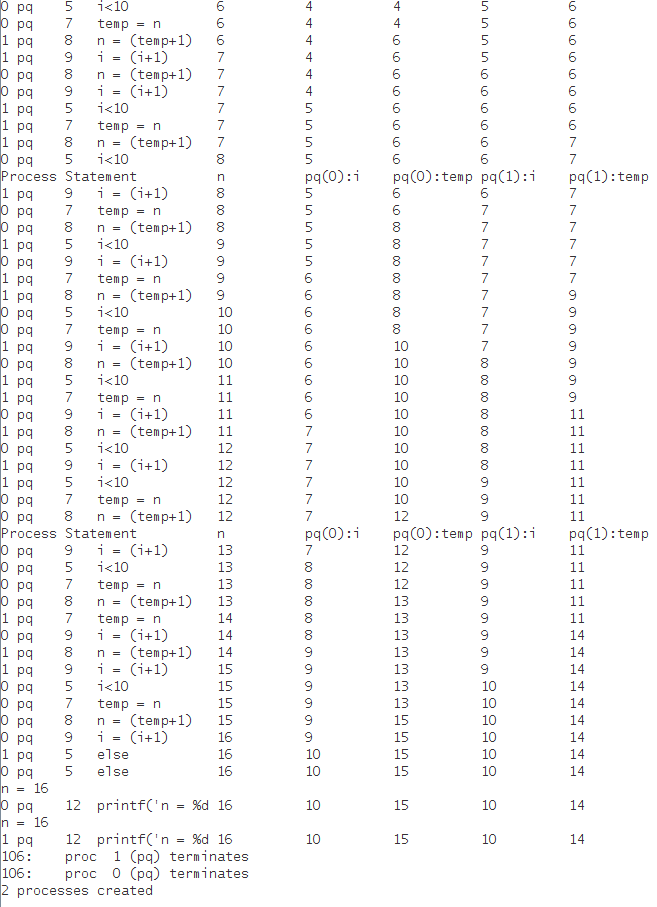
\includegraphics[height=6.7in, width = 6in]{concurrent1.png}\\
\end{center}\\
\newpage
\begin{center}
2. Example with 10 iterations.
\vspace{10mm}

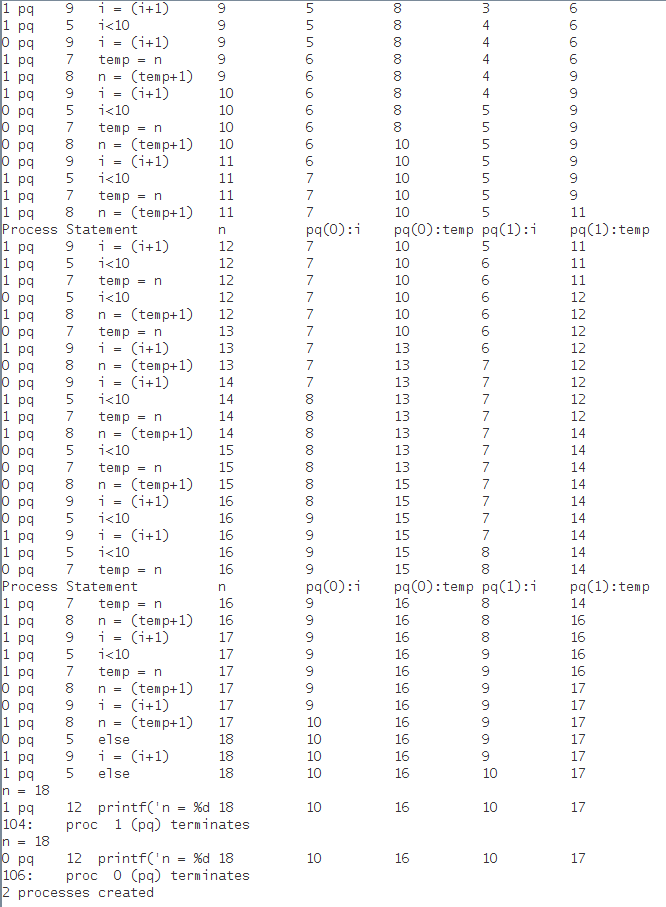
\includegraphics[height=7in, width = 6in]{concurrent2.png}\\
\end{center}\\
\newpage

\begin{center}
3. Example with 10 iterations.
\vspace{10mm}

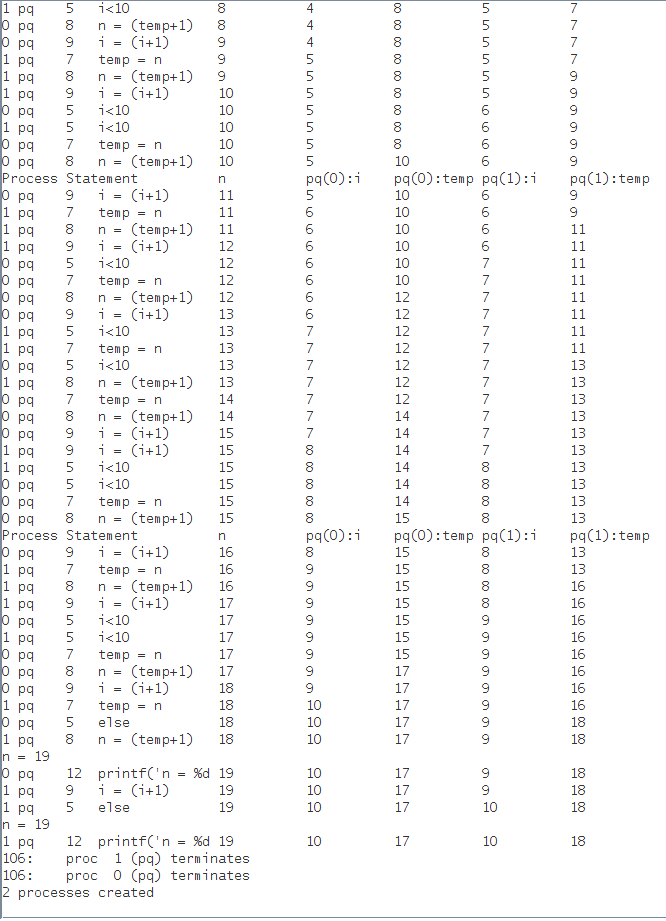
\includegraphics[height=7in, width = 6in]{concurrent3.png}\\
\end{center}\\
\newpage


\section*{Conclusions Problem 2}
\vspace{10 mm}
The conclusion of the examples presented before is that n should be 2 * number of iterations. Well this isn't the value that we print. This happens because the threads are accesing the same value at the same time and it skips incrementations. The part where we increment the value of n it's the critical section of the problem. To avoid this we can use an algorithm like the one presented before, Dekker's algorithm.

\newpage
\section*{References}
https://www.geeksforgeeks.org/dekkers-algorithm-in-process-synchronization/

\end{document}